\documentclass{article}
\usepackage[utf8]{inputenc}
\usepackage{float}
\usepackage{graphicx}
\usepackage{geometry}
\usepackage{tabularx}
\usepackage{acronym}
\usepackage{listings}
\usepackage{lmodern}
\usepackage[version=4]{mhchem}
\usepackage{multicol}
\usepackage{xcolor}

\title{Systems Integration - Assignment \#2}
\date{2019/2020}

\author{João Moreira - 2015230374 \\ 
João Soares - 2009113071 }

\renewcommand{\baselinestretch}{1.3}

\begin{document}

\maketitle

\section{Introduction}

\qquad The intent of this assignment is to develop a web application to manage an online store of secondhand items, called MyBay and deploy it using WildFly Application Server. In order to develop this application, we used Maven to build and manage dependencies and \ac{Java EE}, dividing the system into three layers: presentation, business and data.

\section{Presentation layer}

\qquad To develop the presentation layer we used \ac{JSF} because it is a MVC (model, view, control) framework.

\qquad A non logged in user can only go to the landing page, in this case the login, and access the sign up page, giving him the ability to register in the system and latter login to see the contents of the web-page. This is because we've created a session filter that only gives access to a restricted folder to logged in users. The filter is defined on the web xml.

\qquad In relation to the password storage. We've implemented this system thinking in the security from the front-end, all the way down to the persistence. The actual password never gets transmitted to our application as it goes under a MD5 hash on the clients browser using a JavaScript program, then we pass the hashed password received on more MD5 hashing rounds, so the password saved on the database can't be used to login even if the database information would get exposed.

\qquad After logging in, the user is presented with the home page (figure 1). From this point forward, all the pages use a template created so that they have the same header, giving access to the user to the home, add item and profile page and logout option anywhere on the system. 

\begin{figure}[H]
    \centering
    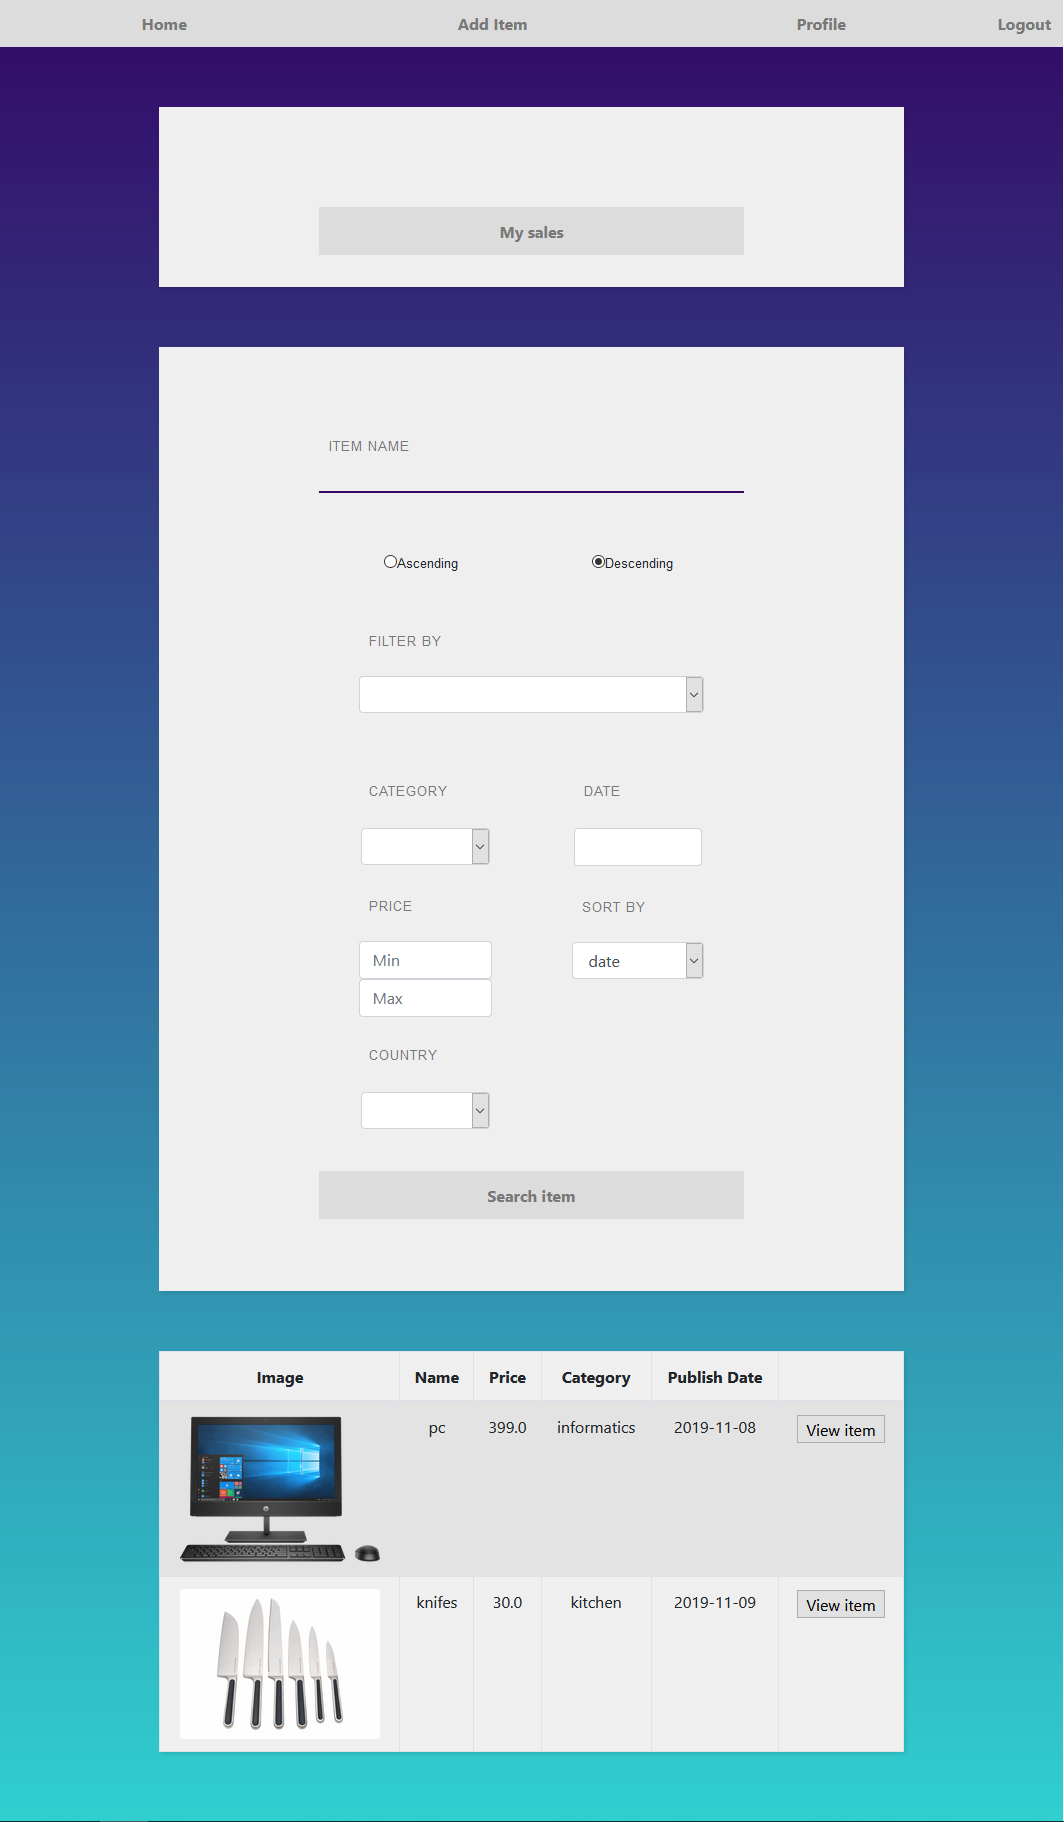
\includegraphics[scale=0.20]{homePage.png}
    \caption{Home page layout after a search.}
   \end{figure}

\qquad In the home page is where the user makes his searches. He's able to search for all items by pressing the "Search item" button, he can see his own items with the button "My sales" and can create various searches by using the input boxes, buttons and drop-down menus.

\qquad The add item section is the place where a new item can be created, and after that, by searching for his own sales, and clicking the view item button, the user can edit and delete his items.

\qquad In the profile area, the user can edit his name, country and password, as well as delete his account, deleting also all of his items for sale.

\qquad By logging out, the session is invalidated, so that the user needs to login again to see all of the pages above. 

\qquad All of the information that the user inserts for searches, updates, etc... is treated in the controllers we've implemented to communicate with the business layer. This controllers call functions that are exposed by the business \ac{EJB}s interfaces and pass information through contracts that are known throughout the system. The item controller is view scoped, the user controller is session scoped and the rest of the controllers implemented are request scoped. 

\qquad One of the most challenging parts of the interface's implementation was the search part. We wanted to make it obvious to the user how the categories to search by are selected, so we made a drop-down menu where the user selects the category he wants to search by. E.g.: I only want to see the items in the category wc. To do that, I need to click filter by, select categories and in the categories drop-down menu select the category wc. After this, I press Search item and will get all items in this category.

\qquad Another challenge was the item's image, resolved with an external API that lets us upload images and gives us the URL and the delete hash, for when the item is removed.



\section{Business layer}

\qquad The connection to the data layer is performed by the business layer, whom has three local stateless \ac{EJB}s implemented. The account, sale and email. They are local because they are running in the same \ac{JVM} as the rest of the system and stateless since we don't need to maintain a conversational state, we only need to perform simple operations. The transactions for this beans are managed by the container, although we don't make any transactions on this layer, the transactions to the database are handled on the level of the data layer.

\qquad On the AccountEJB, most of the information that goes to the presentation layer is boolean, since the operations mainly need confirmations on said layer, exceptionally on the login, where we send the User contract, containing the information's about the user logged in (name, email, encrypted password and country).

\qquad The operations performed by this \ac{EJB} are sign up, login, update account and delete account. This operations send to the data layer the User contract with only the information needed. In the sign up it sends a fully created user (name, email, password and country), in the case of the login just the email and password. For removing the account the email, and for updating it can bring a new name, country or password.

\qquad The SaleEJB, just like the AccountEJB, gathers booleans from the data layer, although, instead of User contracts it collects Item contracts to send to the presentation layer, and sends the mapped information to the presentation layer. The operations performed are create, list, update and delete sales, list an users items for sale and search sales. 

\qquad To send the emails to the users with the three newest items, we have a third \ac{EJB} called EmailEJB, a singleton that initiates upon deployment with a method called newsletter that is scheduled to run every Friday at 8AM. It gets the emails and the three newest items from the data layer (UserEJB and ItemEJB) and sends the emails with this new items through an API. 




\section{Data layer}

\qquad The data layer works atop a database and exposes CRUD functionalities for the \ac{EJB}s ItemEJB and UserEJB. Regarding transactions, we have left the management of all the transactions to the application container and on the data module specified the methods that require a new transaction to run  (mainly all the crud operations) and by default all the \ac{EJB} methods star an implicit transaction when called and end it upon returning from the method.

\qquad We've separated the entities from the persistence layer and the rest of the layers. This is why all the layers only know the user and item object classes that are not persistence entities, doing this we ensured isolation from the persistence entities from the rest of the application maintaining full control over them, performing all persistence operations in this layer.

\qquad To handle all the persistence we used hibernate 5.3 and javax.persistence. 

\qquad We have created interfaces (contracts) to expose the \ac{EJB}s methods and have put them in common modules with the name of the layer, this way the data layer exposes crud, search (to allow the reception of search parameters to refine searches) and list (to perform some list operations). The only layer that has the common data as a dependency is the business layer. This way only in the business layer the data \ac{EJB}s are available. The same was done for the business / web interfaces.

\qquad The database interactions use two other entities to be performed, PersistenceUser and PersistenceItem.  We can see how they interact in the following \ac{ER} (figure 2).

\begin{figure}[H]
 \centering
 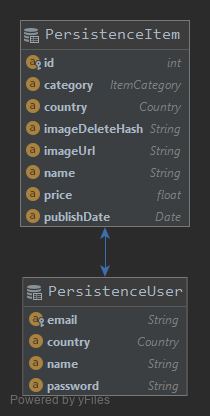
\includegraphics[scale=0.4]{ER_MyBay.png}
 \caption{MyBay \ac{EJB} \ac{ER} diagram.}
 \label{fig:er}
\end{figure}

\qquad Both \ac{EJB}s interface extends the crudable interface and the ItemEJB's extends Searchable, meaning they both implement create, read, update and delete, while user also implements a listing of the user's items for sale and the item implementing a search method that has parameters as it's input.

\qquad In terms of the \ac{EJB} security we have researched the use of role access base (but due to some problems trying to configure the users within WildFly with RBAC and the lack of time we couldn't persue this path)



\section{Project management and packaging}

\qquad All the cycle of (compiling packing and deployment) is done via Maven. The development system was a remote server running WildFly version 18 with java 13 under Ubuntu server 18.04lts. We've performed some configurations to the WildFly server in order to further customize the deployment and inserted the PostgreSQL driver in order to use a database (and configured a data source). Also, we've managed all our dependencies using WildFly. This way we have achieved a small deployment unit.

\qquad The project is divided into 7 folders: common, data, common data, business, common business, web and ear. The common folder has support functions, such as enumerations, converters from and to enumerations and types, it's here where we have the Item and User class used to transfer data between layers. The common data and common business it where we store the interfaces of the \ac{EJB}s of each layer. In the common data we also have the Crudable and Searchable interface. The web, data and business store each of our layers. The ear folder has the pom file that creates the deployable file, packaged has an ear file.

\qquad For logging we used the tool \ac{SLF4J} and created a logging profile to divide the logs by hierarchy and modules. We have a log-file common to all modules that registers all the information and above messages (this way we have a high level view of what's happening within our application). Then we have a separate logging file per module that records all the logs from trace and above, this way if we need to do some more deep investigation of what's happened within the system on a particular layer it's easier. The logging profile is operating in a rolling log file per day of operation.

\qquad Each of our folders has a pom fille. The root pom file has the modules of the project and the dependencies for the project, as well as the WildFly plugin configurations for the server that we're running WildFly on. The web pom has the URL where the system will be accessible from. The rest of the pom filles are used to define the packaging of the modules they're in, in this case both business and data are packaged has ejb, the web module is a war file and the common folders are jar files.\newline\newline






\textbf{Acronym list:}

\begin{acronym}
\acro{JVM}{Java Virtual Machine}
\acro{Java EE}{Java Enterprise Edition}
\acro{JSF}{JavaServer Faces}
\acro{EJB}{Enterprise JavaBeans}
\acro{JPA}{Java Persistence API}
\acro{SLF4J}{Simple Logging Facade for Java}
\acro{ER}{Entity-Relationship}
\acro{RBAC}{Role-Based Access Control}
\end{acronym}

\end{document}
